\section{Première formulation robuste}
\subsection{Modèle}

Afin de prendre en compte les erreurs sur les facteurs d'amplification $x_i$, nous utilisons les valeurs maximales des variations possibles de $\hat{D(\theta)}$ en chaque point de notre discrétisation. Nous imposons que malgré ces variations nous restons dans les intervalles voulus. On transforme par exemple la première contrainte $D(\theta)\leq \epsilon$ du modèle non robuste :
\begin{equation}
d(\theta)^T (x.*(1+\xi)) \leq \epsilon \Longleftrightarrow d(\theta)^T (x.*\xi) \leq \epsilon- d(\theta)^T x
\end{equation}
%Où $d(\theta)$ est le vecteur colonne contenant les $d_i(\theta)$ et $dx(\theta)$ le produit élément par élément de $d(\theta)$ avec $x$.
Nous cherchons à ce que notre optimum $(x,\epsilon)$ soit valable dans le pire cas, c'est-à-dire pour cette contrainte celui où $d(\theta)^T (x.*\xi)$ est maximum. Comme nous imposons également que $|\xi_i|\leq \tau$ nous formulons un problème de maximisation linéaire et imposons une condition sur son objectif: 
\begin{align*}
\max_{\xi_i} d(\theta)^T (x.*\xi)  & \leq \epsilon- d(\theta)^T x \\
\xi_i & \leq \tau \\
-\xi_i & \leq \tau 
\end{align*} 

Nous avons donc un problème d'optimisation dont l'optimum sera inférieur à $\epsilon- d(\theta)^T x $. On peut mettre ce problème sous forme duale. Par dualité forte on sait que l'objectif optimal de ce problème dual sera le même que celui du primal. Celà nous donnera :
\begin{align*}
\min_{y_+,y_-} \mathbf{1}^{n\times 1}\tau y_++\mathbf{1}^{n\times 1}\tau y_- & \leq \epsilon- d(\theta)^T x \\
y_+,y_-  & \geq  0 \\
(I,-I)\begin{pmatrix}
y_+ \\
y_-
\end{pmatrix}
& = 
\begin{pmatrix}
d_1(\theta)x_1 \\
d_2(\theta)x_2 \\
\vdots \\
d_n(\theta)x_n 
\end{pmatrix}
\end{align*}
Comme ce problème est un problème de minimisation, si la contrainte sur l'objectif est satisfaite pour n'importe quelle solution admissible, on sait que l'optimum satisfera aussi cette contrainte.\\
On peut alors revenir à notre problème de base dans lequel on remplace la contrainte $D(\theta)\leq \epsilon$ par les contraintes du dual et la contrainte sur l'objectif.
On traduit de la même manière les autres contraintes. On obtient alors le modèle suivant :

\begin{align*}
\min_{x,\epsilon ,y_1+,y_1-,y_2+,y_2-,y_3+,y_3-,y_4+,y_4-} \epsilon &  \\
y_{i+},y_{i-}  & \geq  0 \\
(I,-I)
 \begin{pmatrix}
y_i+ \\
y_i-
\end{pmatrix}
& = 
\begin{pmatrix}
d_1(\theta)x_1 \\
\vdots \\
d_n(\theta)x_n 
\end{pmatrix} \\
\forall i = 1,2,3,4\:\:
\forall \theta \in S_e \cup P_e  &  \\
\mathbf{1}^{n\times 1}\tau y_{1+}+\mathbf{1}^{n\times 1}\tau y_{1-} & \leq \epsilon -d(\theta)^Tx \\
\mathbf{1}^{n\times 1}\tau y_{2+}+\mathbf{1}^{n\times 1}\tau y_{2-} & \leq \epsilon + d(\theta)^Tx \\
\forall \theta \in S_e &  \\
\mathbf{1}^{n\times 1}\tau y_{3+}+\mathbf{1}^{n\times 1}\tau y_{3-} & \leq  \epsilon +1 -d(\theta)^Tx \\
\mathbf{1}^{n\times 1}\tau y_{4+}+\mathbf{1}^{n\times 1}\tau y_{4-} & \leq  \epsilon -1 + d(\theta)^Tx \\
\forall \theta \in P_e & 
\end{align*}
Cette formulation introduit $8N$ variables supplémentaires par rapport au modèle de base
%TODO : Pourquoi le solver utilise des itérations barrier et pas des simplexes?
\FloatBarrier
\subsection{Analyse des résultats}
Les figures \ref{fig:ModROBUST1} montrent les résultats obtenus pour différentes valeurs de $\tau$. Un récapitulatif des résultats pour les différents modèle est donné à la table \ref{table:Recap}.\\
\begin{itemize}
\item Dans le cas $\tau = 0.001$, on constate une augmentation du $\epsilon$ par rapport au modèle de base. Les erreurs pour les $x_i$ perturbés sont cependant bien moindre. On constate également que les erreurs pour des $x_i$ perturbés avec une perturbation de l'ordre de $\tau=0.001$ ou de $\tau = 0.01$ sont moindre que dans le modèle avec $\tau=0.01$. Cependant, on observe des dépassements pour certaines réalisation des $\xi_i$ si on applique les perturbations de $\tau=0.01$. (ce qui est logique vu que le modèle n'est pas conçu pour résister à de telles perturbations). On constate que l'ordre de grandeur des $x_i$ non-nuls est inférieur à celui du modèle de base ce qui confirme notre intuition comme quoi le modèle robuste a tendance à fournir des $x_i$ plus petits.\\ 
 \item Dans le cas $\tau = 0.01$, on constate toujours une augmentation du $\epsilon$ par rapport au modèle de base et au modèle où $\tau = 0.001$. Les erreurs pour les $x_i$ perturbés sont plus grande que dans le modèle $\tau=0.001$ pour des perturbations de l'ordre de $\tau = 0.001$ et $\tau=0.01$, mais le modèle ne présente jamais de dépassement. On constate que l'ordre de grandeur des $x_i$ non-nuls est inférieur à celui du modèle $\tau=0.001$, ce qui confirme encore notre intuition.
\end{itemize}

\begin{figure}[h!]
  \centering
  \begin{subfigure}[b]{0.32\textwidth}
  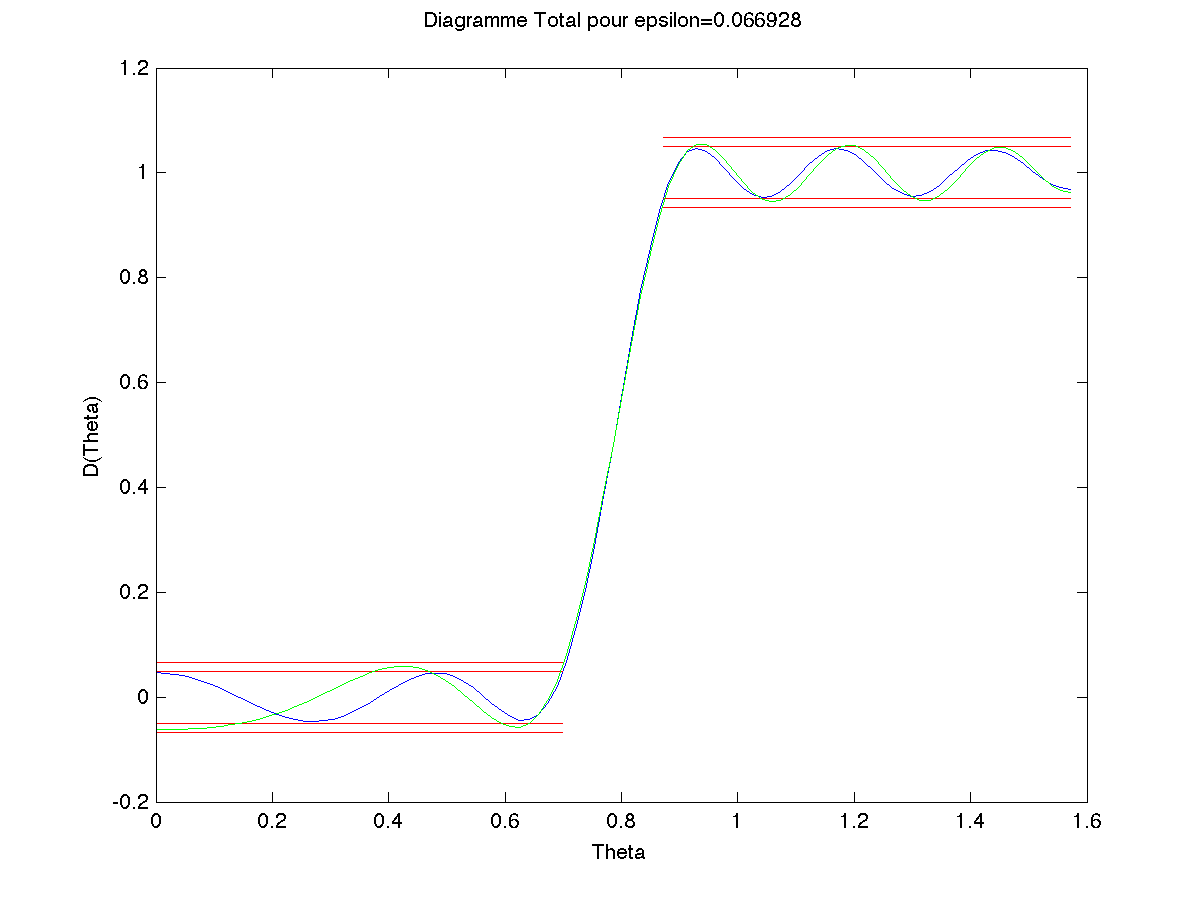
\includegraphics[width=\textwidth]{D-ModRobust1.png}
  \caption{$D(\theta)$ pour le modèle $\tau = 0.01$ (en vert) et $\tau = 0.001$ (en bleu) et $x$ non-perturbé.}
  \label{fig:D-ModRobust1}
  \end{subfigure}
  ~ 
 \begin{subfigure}[b]{0.32\textwidth}
  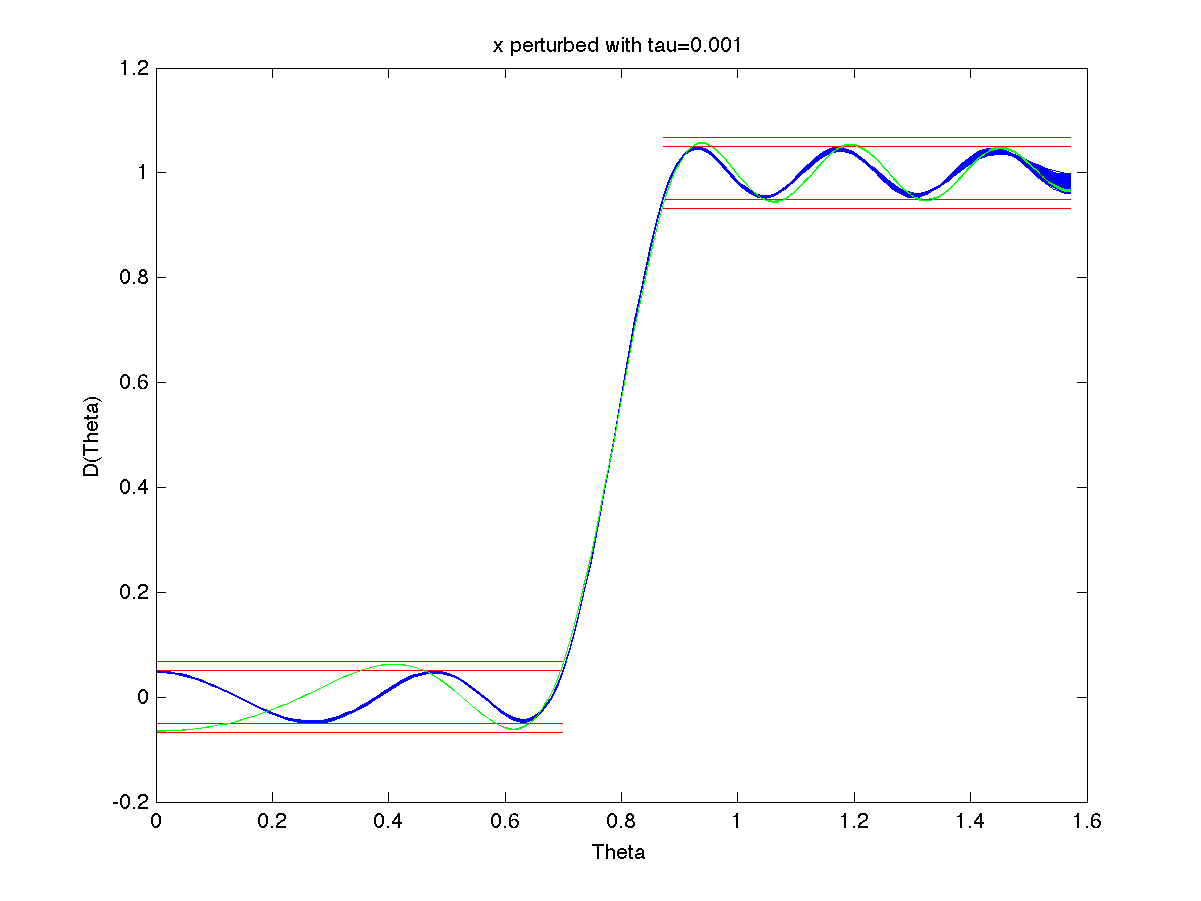
\includegraphics[width=\textwidth]{D-ModRobust1-test3Rob001.png}
  \caption{$D(\theta)$ pour une perturbation de $\tau = 0.001$ sur les $x$ (en vert pour un modèle de $\tau=0.01$ en bleu pour $\tau=0.001$).}
  \label{fig:D-ModRobust1-test3RobTau001}
  \end{subfigure}
  ~ 
  \begin{subfigure}[b]{0.32\textwidth}
  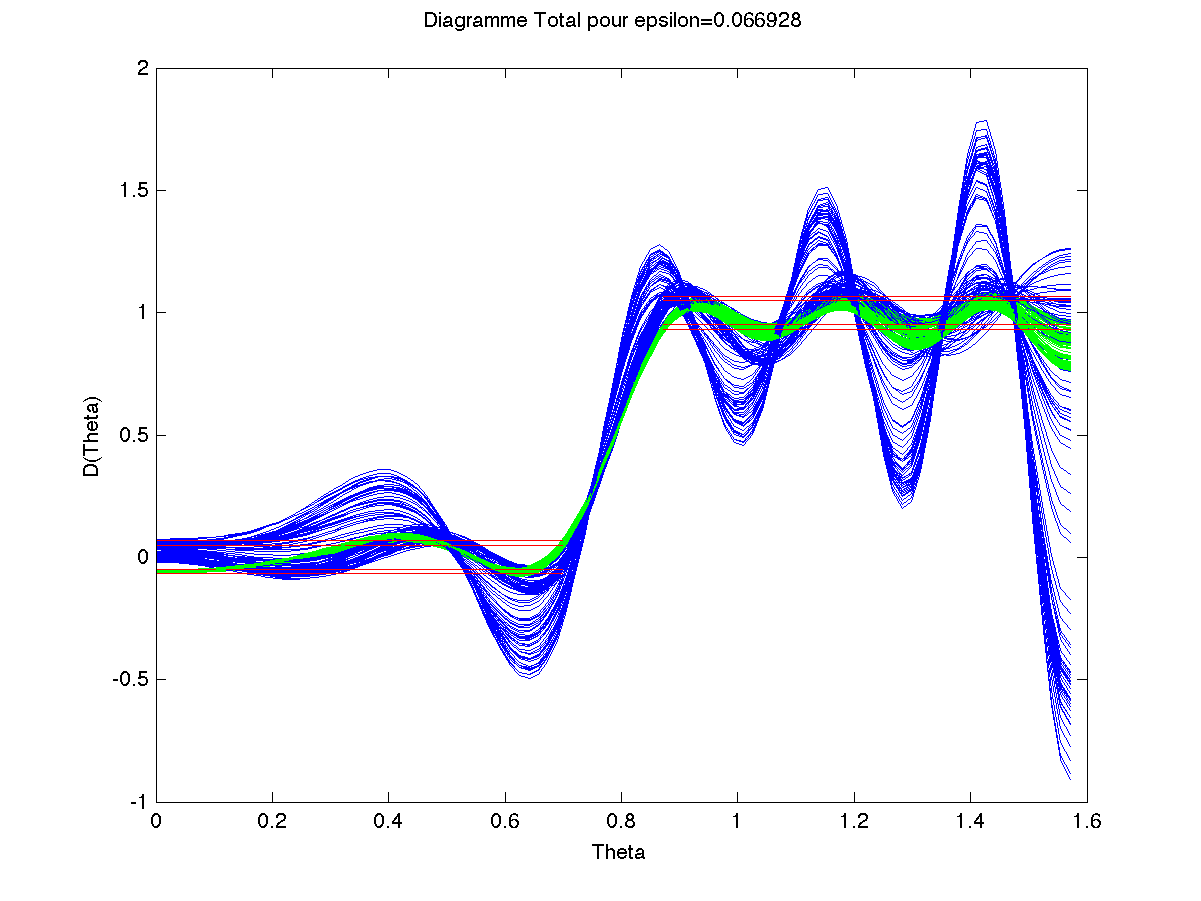
\includegraphics[width=\textwidth]{D-ModRobust1-test3Rob01.png}
  \caption{$D(\theta)$ pour une perturbation de $\tau = 0.01$ sur les $x$ (en vert pour un modèle de $\tau=0.01$ en bleu pour $\tau=0.001$).}
  \label{fig:D-ModRobust1-test3RobTau01}
  \end{subfigure}
\caption{Les deux derniers graphes sont donnés pour une centaine de réalisations des $\xi_i$.}
\label{fig:ModROBUST1}
  \end{figure}

\begin{table}
\centering
\begin{tabular}{c|c|c|ccc}
 & & &  &\textbf{Erreurs pour : } &\\
 & $\epsilon$ & $\mathcal{O}( x_i)$ ($x_i\neq0$ &$x_i$ & $x_i$ pert. ($\tau=0.001$) & $x_i$ pert. ($\tau=0.01$) \\
 \hline
Modèle de base & $2\%$ & $10^3$ &0.0185 & 5.3977 & 47.9054 \\
Modèle robuste 1 ($\tau=0.001$) & $5.07 \%$ & $10^0$& 0.0396 & 0.0396  & 0.0440 \\
Modèle robuste 1 ($\tau=0.01$)  & $6.80 \%$ &$10^{-1}$ &0.0508 & 0.0508 & 0.0510 \\
\end{tabular}
\caption{Récapitulatif des résultats des erreurs et de la borne maximal $\epsilon$ obtenus pour les différents modèles et les différents types de perturbations.}
\label{table:Recap}
\end{table}
\FloatBarrier